\documentclass[a4paper,ngerman,landscape]{scrartcl}

\usepackage[utf8]{inputenc}

\usepackage[ngerman]{babel}
\usepackage{hyperref}

\usepackage{graphicx}

\usepackage[protrusion=true,expansion=true]{microtype}

\usepackage{lmodern}
\usepackage{tabto}

\setlength\parskip{\medskipamount}
\setlength\parindent{0pt}

\usepackage{geometry}
\geometry{tmargin=0.5cm,bmargin=0.0cm,lmargin=2.5cm,rmargin=2.5cm}

\pagestyle{empty}

\begin{document}

\begin{center}
  \Huge
  Mittwoch, 21. August 2013, 10:00 Uhr, 2004/L1 \\
  \textbf{Ingo Blechschmidt: Konstruktive Mathematik II}
  \vfill
  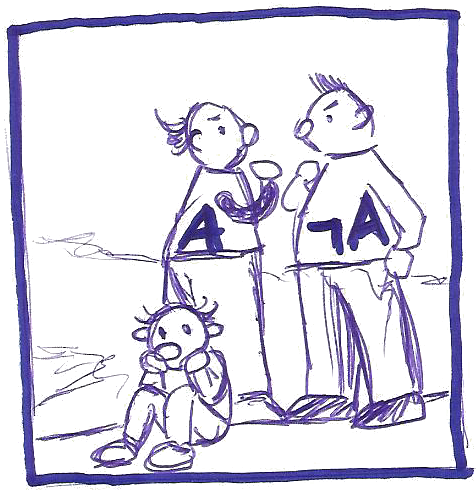
\includegraphics[scale=1.6]{lem}
  \vfill

  \Large
  \begin{minipage}{0.91\textwidth}
    \setlength\parskip{\medskipamount}
    Im ersten Vortrag hatten wir konstruktive Mathematik kennengelernt, das ist
    Mathematik ohne Verwendung des Prinzips vom ausgeschlossenen Dritten,
    sodass Widerspruchsbeweise nicht pauschal zulässig sind. Nun wollen wir
    die sog. \emph{Doppelnegationsübersetzung} verstehen, die eine Beziehung
    zur klassischen Logik herstellt und die geschichtliche Relevanz
    konstruktiver Methoden im Rahmen von \emph{Hilberts Programm} aufzeigt.
    Dabei werden wir auf eine tiefgründige Verbindung zur theoretischen
    Informatik stoßen und eine Parabel über einen König, einen Philosophen und den Stein der
    Weisen diskutieren.
  \end{minipage}
\end{center}

\newpage

\begin{center}
  \Huge
  Mittwoch, 21. August 2013, 12:15 Uhr, 2004/L1 \\
  \textbf{Tim Baumann und Carina Willbold: Singulärwertzerlegung und
  Hauptkomponentenanalyse}
  \vfill
  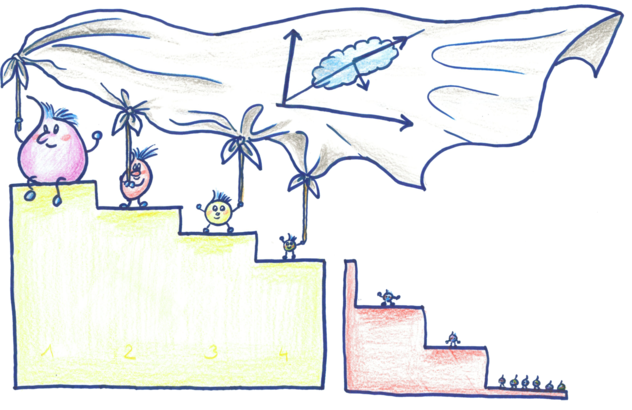
\includegraphics[scale=0.75]{svd}
  \vfill

  \Large
  \begin{minipage}{0.91\textwidth}
    \setlength\parskip{\medskipamount}
    Jede reelle oder komplexe Matrix erlaubt eine sog.
    \emph{Singulärwertzerlegung}, in Verallgemeinerung der bekannten
    Eigenwertzerlegung, die bekanntlich nur für quadratische und
    diagonalisierbare Matrizen möglich ist. Im Vortrag werden wir nach einer
    theoretischen Einführung interaktiv zwei ihrer vielfältigen Anwendungen
    kennenlernen: die Approximation von Matrizen durch welche mit viel
    kleinerem Rang (nützlich etwa für Bildkompression) und die
    Hauptkomponentenanalyse (nützlich für statistische Datenanalyse).
  \end{minipage}
\end{center}
\end{document}
